\documentclass[a4paper]{amsart}

%                  Trash .aux file after toggling
\usepackage{stmaryrd}
\usepackage{graphicx}
\usepackage[margin=1in]{geometry}
\usepackage[lutzsyntax]{virginialake}\aftrianglefalse
\usepackage[pdfborder={0 0 0}]{hyperref}

%--------- Theorem etc
\newtheorem{thm}{Theorem}[section]
\newtheorem{cor}[thm]{Corollary}
\newtheorem{lem}[thm]{Lemma}
\newtheorem{pro}[thm]{Proposition}

\theoremstyle{remark}
\newtheorem{rem}[thm]{Remark}

\theoremstyle{definition}
\newtheorem{defi}[thm]{Definition}
%---------

%-------------------------------------------------------- REMOVE WHEN PAPER DONE
\newcommand{\Ale}[1]{{\color{red}\noindent {\bf A:} #1}}
\newcommand{\Tom}[1]{{\color{green}\noindent {\bf T:} #1}}
\newcount\todocount\todocount=0
\newcommand{\TODO}[1]{\global\advance\todocount by1%
            {\color{red}\noindent{\bf\the\todocount\ TODO:} #1}}\vlupdate{\TODO}
\renewcommand{\Ale}[1]{\relax}  % Comment/uncomment these three lines
\renewcommand{\Tom}[1]{\relax}  % in order to display/hide inline comments
%\renewcommand{\TODO}[1]{\relax} %
%-------------------------------------------------------- REMOVE WHEN PAPER DONE

\begin{document}

\title[Normalisation Control in Deep Inference   via Atomic Flows II]
      {Normalisation Control in Deep Inference\\ via Atomic Flows II}

\author{Alessio Guglielmi and Tom Gundersen}
%\address{University of Bath, Bath BA2 7AY, UK}

\thanks{This work was in part funded by an Overseas Research Scholarship and a Research Studentship, both from the University of Bath, and by the British Council Alliance Programme.}

\keywords{Normalisation, deep inference, cut elimination, atomic flows}

\subjclass{F.4.1 Mathematical Logic---Proof theory}

% \begin{abstract}
% \end{abstract}

\maketitle

%===============================================================================
\section{Background on Deep Inference}

Deep inference is a relatively recent development in proof theory. It is a methodology according to which several formalisms can be defined with excellent structural properties. The calculus of structures \cite{Gugl:06:A-System:kl} is one of them and is now well developed for classical \cite{Brun:03:Atomic-C:oz,Brun:06:Cut-Elim:cq,Brun:06:Locality:zh,BrunTiu:01:A-Local-:mz,Brun:06:Deep-Inf:qy}, intuitionistic \cite{Tiu:06:A-Local-:gf}, linear \cite{Stra:02:A-Local-:ul,Stra:03:MELL-in-:oy}, modal \cite{Brun::Deep-Seq:ay,GoreTiu:06:Classica:uq,Stou:06:A-Deep-I:rt} and commutative/non-commutative logics \cite{Gugl:06:A-System:kl,Tiu:06:A-System:ai,Stra:03:Linear-L:lp,Brus:02:A-Purely:wd,Di-G:04:Structur:wy,GuglStra:01:Non-comm:rp,GuglStra:02:A-Non-co:lq,GuglStra:02:A-Non-co:dq,Kahr:06:Reducing:hc,Kahr:07:System-B:fk}. The basic proof complexity properties of the calculus of structures are known \cite{BrusGugl:07:On-the-P:fk}. The calculus of structures promoted the discovery of a new class of proof nets for classical and linear logic \cite{LamaStra:05:Construc:qq,LamaStra:05:Naming-P:ov,LamaStra:06:From-Pro:et,StraLama:04:On-Proof:ec} (see also \cite{Guir:06:The-Thre:qt}). There exist implementations in Maude of deep-inference proof systems \cite{Kahr:07:Maude-as:lr}. For a better introduction than this, we refer the reader to \cite{Brun:03:Atomic-C:oz}.

\newcommand{\fff}{\mathsf f}
\newcommand{\ttt}{\mathsf t}
\newcommand{\ot}{\mathbin\shortleftarrow}

%---------------------------------------
\begin{defi}
\emph{Formulae}, $\alpha$, $\beta$, $\gamma$, $\delta$ are freely built from: \emph{units}, $\fff$ (false), $\ttt$ (true); \emph{atoms}, $a$, $b$, $c$, $d$, $e$; \emph{disjunction} and \emph{conjunction}, ${\vlsbr[\alpha.\beta]}$ and $\vlsbr(\alpha.\beta)$. On the set of atoms a (non-identical) involution $\bar\cdot$ is defined, and dual atom occurrences, as $a$ and $\bar a$, can appear in formulae. We denote \emph{contexts}, \emph{i.e.}, formulae with a hole, by $\xi\vlhole$ and $\zeta\vlhole$; we also use \emph{multiple} contexts, $\xi\vlhole\cdots\vlhole$, \emph{i.e.}, formulae with many holes; for example, if $\xi\{a\}$ is $\vls(b.[a.c])$, then $\xi\vlhole$ is $\vls(b.[\vlhole.c])$, $\xi\{b\}$ is $\vls(b.[b.c])$ and $\xi\vlscn(a.d)$ is $\vls(b.[(a.d).c])$; if $\xi\{a\}\{b\}\{c\}$ is $\vls(b.[(a.d).c])$ then $\xi\{b\}\{c\}\{a\}$ is $\vls(c.[(b.d).a])$.
\end{defi}

%---------------------------------------
\begin{rem}
Negation is only defined for atoms, which is not a limitation thanks to De Morgan laws.
\end{rem}

Note that when we write $\xi\{a\}$, we mean that an occurrence of $a$ exists in the formula, we singled it out and we refer specifically to that occurrence. It is important to distinguish between an atom $a$ and a set of occurrences of atom $a$ inside a formula or a derivation. In the following, we mark in various ways occurrences of atoms, and we perform several substitutions of formulae in the place of atom occurrences.

\newcommand{\one}{{\mathchoice{\scriptstyle\mathbf1}
                              {\scriptstyle\mathbf1}
                              {\scriptstyle\mathbf1}
                              {\scriptscriptstyle\mathbf1}}}
\newcommand{\two}{{\mathchoice{\scriptstyle\mathbf2}
                              {\scriptstyle\mathbf2}
                              {\scriptstyle\mathbf2}
                              {\scriptscriptstyle\mathbf2}}}
\newcommand{\mk}[1]{{#1}^{\scriptscriptstyle\bullet}}
%---------------------------------------
\begin{defi}
\emph{Inference rules}, $\rho$, have one \emph{premiss} and one \emph{conclusion}, and their \emph{instances} are used in \emph{inference steps} to rewrite inside formulae. A \emph{derivation}, $\Phi$, from $\alpha$ (\emph{premiss}) to $\beta$ (\emph{conclusion}) is a chain of inference steps with $\alpha$ at the top and $\beta$ at the bottom, and is usually indicated by $\vlder{\Phi}{\mathcal S}{\beta}{\alpha}$, where $\mathcal S$ is the name of the deductive system or a set of inference rules; a \emph{proof} is a derivation from $\ttt$; besides $\Phi$, we denote derivations with $\Psi$. We denote with $\xi\{\Phi\}$ the result of including every formula of the derivation $\Phi$ from $\alpha$ to $\beta$ into the context $\xi\vlhole$: since we adopt deep inference, $\xi\{\Phi\}$ from $\xi\{\alpha\}$ to $\xi\{\beta\}$ is a valid derivation. Furthermore, $\xi\left\{\vlder{}{}{\beta_1}{\alpha_1}\right\}\cdots\left\{\vlder{}{}{\beta_n}{\alpha_n}\right\}$ denotes the concatenation of $\xi\left\{\vlder{}{}{\beta_1}{\alpha_1}\right\}\{\alpha_2\}\cdots\{\alpha_n\},\dots,\xi\{\beta_1\}\cdots\{\beta_{n-1}\}\left\{\vlder{}{}{\beta_n}{\alpha_n}\right\}$. We denote with $\Phi\{a\ot\alpha\}$ the operation of substituting $\alpha$ into a set of \emph{occurrences} of an atom $a$ in $\Phi$; the result is not necessarily a valid derivation, because some instances of rules might break; which occurrences to replace is always made clear by suitable decorations of $a$, like $a^\star$.
\end{defi}

\newcommand{\KS}{\mathsf{KS}}
\newcommand{\SKS}{\mathsf{SKS}}
Now we define the two standard deductive systems for classical propositional logic in deep inference that are used throughout the paper. $\KS$ is analytic, in the sense that premisses only contain subformulae of conclusions, and $\SKS$ is not \cite{Brun:03:Atomic-C:oz,Brun:06:Cut-Elim:cq,Brun:06:Locality:zh,BrunTiu:01:A-Local-:mz}.

\newcommand{\ai}{\mathsf{ai}}
\newcommand{\aw}{\mathsf{aw}}
\newcommand{\ac}{\mathsf{ac}}
\newcommand{\aid}{{\ai{\downarrow}}}
\newcommand{\awd}{{\aw{\downarrow}}}
\newcommand{\acd}{{\ac{\downarrow}}}
\newcommand{\aiu}{{\ai{\uparrow}}}
\newcommand{\awu}{{\aw{\uparrow}}}
\newcommand{\acu}{{\ac{\uparrow}}}
\newcommand{\swi}{\mathsf{s}}
\newcommand{\med}{\mathsf{m}}
%---------------------------------------
\begin{defi}
System $\SKS$ in the calculus of structures is defined by the following \emph{structural} rules:
\[
\begin{array}{@{}c@{}c@{}c@{}}
      \vlinf{\aid}{}{\vls[a.{\bar a}]}{\ttt}&
\qquad\vlinf{\awd}{}a\fff&
\qquad\vlinf{\acd}{}a{\vls[a.a]}\\
\noalign{\smallskip}
      \emph{interaction}&
\qquad\emph{weakening}&
\qquad\emph{contraction}\\
\noalign{\bigskip}
      \vlinf{\aiu}{}\fff{\vls(a.{\bar a})}&
\qquad\vlinf{\awu}{}\ttt a&
\qquad\vlinf{\acu}{}{\vls (a.a)}a\\
\noalign{\smallskip}
      \emph{cointeraction}&
\qquad\emph{coweakening}&
\qquad\emph{cocontraction}\\
\end{array}\quad,
\]
and by the two \emph{logical} rules:
\[
\begin{array}{@{}c@{}c@{}}
\vlinf{\swi}{}{\vls[(\alpha.\beta).\gamma]}{\vls(\alpha.[\beta.\gamma])}&\qquad
\vlinf{\med}{}{\vls([\alpha.\gamma].[\beta.\delta])}
              {\vls[(\alpha.\beta).(\gamma.\delta)]}\\
\noalign{\smallskip}
\emph{switch}&\qquad\emph{medial}\\
\end{array}\quad.
\]
The rule cointeraction is also called an (\emph{atomic}) \emph{cut}. In addition to the rules shown, there is a rule $\vldownsmash{\vlinf={}\delta\gamma}$, such that $\gamma$ and $\delta$ are opposite sides in one of the following equations:
\vlstore{
\vls[\alpha.\beta]         &=\vls[\beta.\alpha]         \quad,&
\vls[\alpha.\fff]          &=\vls[\alpha]               \quad,\\
\vls(\alpha.\beta)         &=\vls(\beta.\alpha)         \quad,&
\vls(\alpha.\ttt)          &=\vls(\alpha)               \quad,\\
\vls[[\alpha.\beta].\gamma]&=\vls[\alpha.[\beta.\gamma]]\quad,&
\vls[\ttt.\ttt]            &=\vls[\ttt]                 \quad,\\
\vls((\alpha.\beta).\gamma)&=\vls(\alpha.(\beta.\gamma))\quad,&
\vls(\fff.\fff)            &=\vls(\fff)                 \quad\vldot}
\begin{align*}
\vlread
\end{align*}
We do not always show the instances of rule $=$, and when we do show them, we gather several contiguous instances into one. System $\KS$ is the same as $\SKS$, but without the rules $\aiu$, $\awu$ and $\acu$. A \emph{cut-free} derivation is a derivation where $\aiu$ is not used. All derivations in this paper are in $\SKS$, unless indicated otherwise.
\end{defi}

Note that all the structural rules only apply to atoms. As shown later, equivalent structural rules applying to formulae instead of atoms can be derived from the atomic ones together with the logical rules. The fact that we can work only with atomic structural rules is essential later on.

Instead of the term `axiom' we use `interaction'; the reason is that, in deep inference, axioms do not close derivation branches. However, it is not misleading to think of interaction instances as axiom instances in the sequent calculus. In several papers, including \cite{Brun:03:Atomic-C:oz}, the reader can find explanations of how reducing a proof in $\SKS$ to a proof in $\KS$ is a cut-elimination process in the traditional sense. In other words, the rules $\aiu$, $\awu$ and $\acu$ are, together, morally equivalent to a cut in the sequent calculus.


%===============================================================================
% \section{Introduction}
% \newcommand{\ot}{\mathbin\shortleftarrow}
% \newcommand{\fff}{\mathsf f}
% \newcommand{\ttt}{\mathsf t}
% \newcommand{\ai}{\mathsf{ai}}
% \newcommand{\aw}{\mathsf{aw}}
% \newcommand{\ac}{\mathsf{ac}}
% \newcommand{\aid}{{\ai{\downarrow}}}
% \newcommand{\awd}{{\aw{\downarrow}}}
% \newcommand{\acd}{{\ac{\downarrow}}}
% \newcommand{\aiu}{{\ai{\uparrow}}}
% \newcommand{\awu}{{\aw{\uparrow}}}
% \newcommand{\acu}{{\ac{\uparrow}}}
% \newcommand{\swi}{\mathsf{s}}
% \newcommand{\med}{\mathsf{m}}
% \newcommand{\sus}{\mathsf{ss}}
% \newcommand{\said}{\mathsf{s}\aid}
% \newcommand{\SKS}{\mathsf{SKS}}
% \newcommand{\KS}{\mathsf{KS}}
% \newcommand{\ppl  }{{\mathchoice{\scriptstyle+}
%                                 {\scriptstyle+}
%                                 {\scriptstyle+}
%                                 {\scriptscriptstyle+}}}
% \newcommand{\pmi  }{{\mathchoice{\scriptstyle-}
%                                 {\scriptstyle-}
%                                 {\scriptstyle-}
%                                 {\scriptscriptstyle-}}}
%---------------------------------------
\section{Preliminaries}
\begin{lem}\label{LemSuperSwitch}
Given a context $\xi\vlhole$ and a formula $\alpha$ there exist derivations $\vlder{}{\{\swi\}}{\xi\{\alpha\}}{\vls(\alpha.\xi\{\ttt\})}$ and $\vlder{}{\{\swi\}}{\vls[\xi\{\fff\}.\alpha]}{\xi\{\alpha\}}$.
\end{lem}

\begin{proof}
We show how to construct the first derivation, the second one can be done by symmetry. We argue by induction on the number of atoms in $\xi\vlhole$. There are three cases to consider, where $\beta$ is not a unit:
\begin{itemize}
  \item $\xi\vlhole=\vlhole$,
  \item $\xi\vlhole=\vls[\xi'\vlhole.\beta]$,
  \item $\xi\vlhole=\vls(\xi'\vlhole.\beta)$.
\end{itemize}

For each case we can build the required derivation:

\[
\vlinf{=}{}{\alpha}{\vls(\alpha.\ttt)}\quad,\qquad
\vlderivation
{
 \vlin{\swi}{}{\vls[\vlder{\Psi}{\{\swi\}}{\xi'\{\alpha\}}{\vls(\alpha.\xi'\{\ttt\})}.\beta]}
 {
  \vlhy{\vls(\alpha.[\xi'\{\ttt\}.\beta])}
 }
}\qquad\mbox{and}\qquad
\vlderivation
{
 \vlin{=}{}{\vls(\vlder{\Psi'}{\{\swi\}}{\xi'\{\alpha\}}{\vls(\alpha.\xi'\{\ttt\})}.\beta)}
 {
  \vlhy{\vls(\alpha.(\xi'\{\ttt\}.\beta))}
 }
}\quad,
\]
where $\Psi$ and $\Psi'$ exists by the inductive hypothesis.
\end{proof}

\begin{lem}\label{LemContr}
Given a formula $\alpha$ and a positive integer $n$, there exist derivations $\vlder{}{\{\acd,\med\}}{\alpha}{\bigvee_{i=1}^{n}\alpha}$\\ and $\vlder{}{\{\acu,\med\}}{\bigwedge_{i=1}^{n}\alpha}{\alpha}$.
\end{lem}

%TODO: Need to get rid of cuts that are not connected to axioms

\begin{defi}
Given a derivation $\Phi$ from $\alpha$ to $\beta$, where $a_1,\dots,a_n$ are all the distinct atoms that appear in both interaction and cointeraction instances, a \emph{core of\ $\Phi$} is defined as a derivation 
\[
\vlder{}{}{\vls[\beta.(a_n.\bar a_n).\cdots.(a_1.\bar a_1)]}{\vls([a_1.\bar a_1].\cdots.[a_n.\bar a_n].\alpha)}
\]
where the atoms $a_1,\dots,a_n$ do not occur in any interaction nor cointeraction instances.
\end{defi}

\begin{lem}\label{LemConstrCore}
Given a derivation $\Phi$ from $\alpha$ to $\beta$, a core of $\Phi$ can be constructed.
\end{lem}

\begin{proof}
Let $a_1,\dots,a_n$ be all the atoms that occur in both interaction and cointeraction instances in $\Phi$. Obtain $\Phi'$ from $\Phi$ by using Lemma~\ref{LemSuperSwitch} to perform the following transformation for each instance of $\aid$ and $\aiu$ applied to $a$ from $a_1,\dots,a_n$ in $\Phi$:
\[
\vlderivation
{
 \vlde{\Psi'}{}{\beta}
 {
  \vlin{\aid}{}{\xi\vlsbr[a.{\bar a}]}
  {
   \vlde{\Psi}{}{\xi\{\ttt\}}
   {
    \vlhy{\alpha}
   }
  }
 }
}\quad\rightarrow\quad
\vlderivation
{
 \vlde{\Psi'}{}{\beta}
 {
  \vlde{}{\{\swi\}}{\xi\vlsbr[a.{\bar a}]}
  {
   \vlhy{\vlsbr([a.{\bar a}].\vlder{\Psi}{}{\xi\{\ttt\}}{\alpha})}
  }
 }
}\qquad\mbox{and}\qquad
\vlderivation
{
 \vlde{\Psi'}{}{\beta}
 {
  \vlin{\aid}{}{\xi\{\fff\}}
  {
   \vlde{\Psi}{}{\xi\vlsbr(a.{\bar a})}
   {
    \vlhy{\alpha}
   }
  }
 }
}\quad\rightarrow\quad
\vlderivation
{
 \vlde{}{\{\swi\}}{\vlsbr[\vlder{\Psi'}{}{\beta}{\xi\{\fff\}}.(a.{\bar a})]}
 {
  \vlde{\Psi}{}{\xi\vlsbr(a.{\bar a})}
  {
   \vlhy{\alpha}
  }
 }
}\quad.
\]

Obtain the core of $\Phi$ from $\Phi'$ by using Lemma~\ref{LemContr}:
\[
\vlderivation
{
 \vlde{}{\{\acd,\med\}}{\vls[\beta.(a_n.{\bar a_n}).\cdots.(a_1.{\bar a_1})]}
 {
  \vlde{\Phi'}{}{\vls[\beta.(a_n.\bar a_n).\cdots.(a_n.\bar a_n).\cdots.(a_1.\bar a_1).\cdots.(a_1.\bar a_1)]}
  {
   \vlde{}{\{\acu,\med\}}{\vls([a_1.\bar a_1].\cdots.[a_1.\bar a_1].\cdots.[a_n.\bar a_n].\cdots.[a_n.\bar a_n].\alpha)}
   {
    \vlhy{\vls([a_1.{\bar a_1}].\cdots.[a_n.{\bar a_n}].\alpha)}
   }
  }
 }
}\quad.
\]
\end{proof}

\newcommand{\Core}{\mathsf{Core}}

\begin{defi}
A core of a derivation $\Phi$ constructed as described in the proof of Lemma~\ref{LemConstrCore} is called \emph{the canonical core of $\Phi$}, written $\Core(\Phi)$.
\end{defi}


\section{Experiments}


% TODO: the definition of cone is wrong...

\begin{defi}
Given a derivation $\Phi$ containing the atom occurence $a$,
\begin{itemize}
 \item if $a$ is in the conclusion of an inference rule $\rho$ and $\sigma$ is a minimal renaming which renames $a$ and preserves the validity of $\rho$, then the \emph{predecessors of $a$} are the atom occurences in the premiss of $\rho$ which are renamed by $\sigma$,
 \item the \emph{cone of $a$} is the set containing $a$ and the cones of the predecessors of $a$.
\end{itemize}
\end{defi}

\begin{defi}
Given a derivation $\Phi$ from $\alpha$ to $\beta$ and, $a_1,\dots,a_n$, a choice of either $a$ or $\bar a$ for each atom occuring in a cointeraction instance in $\Phi$ an \emph{experiment on $\Phi$ with respect to $a_1,\dots,a_n$} is a derivation from $\vls(\bar a_1.\cdots.\bar a_n)$ to $\beta$ which does not contain any interaction nor cointeraction instances and which has the same size as $\Phi$ up to a polynomial.
\end{defi}

\begin{lem}\label{LemConstrExp}
Given a derivation $\Phi$ from $\alpha$ to $\beta$ and, $a_1,\dots,a_n$, a choice of either $a$ or $\bar a$ for each atom occuring in a cointeraction instance in $\Phi$. There exists an experiment on $\Phi$ with respect to $a_1,\dots,a_n$.
\end{lem}

\begin{proof}
\begin{figure}[tbp]
\[
\begin{array}{c}
\vlinf{\awd}{}{a^\star}{\fff}
\quad\rightarrow\quad
\vlinf{=}{}{\fff}{\fff}
\\
\noalign{\bigskip}
\vlinf{\acd}{}{a^\star}{\vls[a^\star.a^\star]}
\quad\rightarrow\quad
\vlinf{=}{}{\fff}{\fff}
\\
\noalign{\bigskip}
\vlinf{\acu}{}{\vls(a^\star.a)}{a^\star}
\quad\rightarrow\quad
\vlinf{\awd}{}{a}{\fff}
\end{array}
\]
\label{FigConeRed}
\end{figure}%

Mark the cones of the atom occurences in the conclusion of $\Core(\Phi)$ which are not in $\beta$ and which are in $a_1,\dots,a_n$ with $\star$. Then perform the following substitutions to obtain $\Core(\Phi)^\star$:
\begin{itemize}
  \item substitute each occurence of $a^\star$ with $\fff$ and
  \item substitute each structural inference rule applied to $a^\star$ as shown in Table~\ref{FigConeRed}.
\end{itemize}
Finally apply $\awu$ to all the atom occurences in the conclusion of $\Core(\Phi)^\star$ which are not in $\beta$ to obtain the experiment:
\[
\vlderivation
{
 \vlde{\Core(\Phi)\{a_1^\star\ot\fff,\dots,a_n^\star\ot\fff\}}{}{\vls[\beta.(\vlinf{\awu}{}{\ttt}{\bar a_1}.\fff).\cdots.(\vlinf{\awu}{}{\ttt}{\bar a_n}.\fff)]}
 {
  \vlhy{\vls(\bar a_1.\cdots.\bar a_n)}
 }
}
\]
\end{proof}

\newcommand{\Exp}{\mathsf{Exp}}

\begin{defi}
An experiment on a derivation $\Phi$ with respect to $a_1,\dots,a_n$ constructed as described in the proof of Lemma~\ref{LemConstrExp} is called \emph{the canonical experiment on $\Phi$ with respect to $a_1,\dots,a_n$}, written $\Exp(\Phi,a_1,\dots,a_n)$.
\end{defi}

%TODO: define canonical

\begin{lem}
Given a set of atoms of size $2n$ closed under negation. Consider an enumeration, $A_n$, of all the possible chocies of $n$ distinct, non-dual atoms from this set. Then $\bigvee_{\{a_1,\dots,a_n\}\in A_n}\vls(a_1.\cdots.a_n)$ is a tautology with a canonical proof in $\{\aid,\acu,\med,\swi\}$.
\end{lem}

\begin{proof}
Argue by induction on $n$. The base case, $n=0$, is trivial and the inductive case is:
\[
\vlderivation
{
 \vlin{=}{}{\bigvee_{\{a_1,\dots,a_k\}\in A_k}\vls(a_1.\cdots.a_k)}
 {
  \vlde{}{\{\swi\}}{\bigvee_{\{a_1,\dots,a_{k-1}\}\in A_{k-1}}\vls[(a_1.\cdots.a_{k-1}.a_k).(a_1.\cdots.a_{k-1}.\bar a_k)]}
  {
   \vlde{}{\{\swi\}}{\bigvee_{\{a_1,\dots,a_{k-1}\}\in A_{k-1}}\vls([a_k.\bar a_k].(a_1.\cdots.a_{k-1}).(a_1.\cdots.a_{k-1}))}
   {
    \vlde{}{\{\med,\acu\}}{\vls(\bigwedge_{i=1}^{2^{k-1}}[a_k.\bar a_k].\bigvee_{\{a_1,\dots,a_{k-1}\}\in A_{k-1}}\vls((a_1.\cdots.a_{k-1}).(a_1.\cdots.a_{k-1})))}
    {
     \vlin{\aid}{}{\vls([a_k.\bar a_k].\bigvee_{\{a_1,\dots,a_{k-1}\}\in A_{k-1}}(a_1.\cdots.a_{k-1}))}
     {
      \vlhy{\bigvee_{\{a_1,\dots,a_{k-1}\}\in A_{k-1}}\vls(a_1.\cdots.a_{k-1})}
     }
    }
   }
  }
 }
}\quad.
\]
Notice that the conclusion consists of the same number of occurences of each atom and every atom occurs in exactly one interaction instance. It follows that each atom occurs in the same number of cocontraction instances and hence the atomic flow of each atom is the same and the proof is canonical.
\end{proof}

%TODO: Define SKS and KS

\begin{thm}
Given a proof, $\Phi$, of $\alpha$ in $\SKS$ there exists a canonical proof of $\alpha$ in $\SKS\setminus\{\aiu\}$.
\end{thm}

\begin{proof}
Let $\{a_1,\dots,a_n,\bar a_1,\dots,\bar a_n\}$ be the set of atoms in $\Phi$ which occur in cointeraction instances and let $A$ be an enumeration of all the possible chocies of $n$ distinct, non-dual atoms from this set. Now build the canonical derivation:
\[
\vlderivation
{
 \vlde{}{\{\acd,\med\}}{\alpha}
 {
  \vlpr{}{\{\aid,\acu,\swi,\med\}}{\bigvee_{\{a_1,\dots,a_n\}\in A}\vlder{\Exp(\Phi,a_1,\dots,a_n)}{\SKS\setminus\{\aid,\aiu\}}{\alpha}{\vls(a_1.\cdots.a_n)}}
 }
}
\]
\end{proof}

\begin{cor}
Given a proof of $\alpha$ in $\SKS$ there exists a canonical proof of $\alpha$ in $\KS$.
\end{cor}


%===============================================================================
\section{Normaliser}

\newcommand{\Norm}{\mathsf{Norm}}

\begin{defi}
The \emph{normaliser}, $\Norm(\Phi,a_1,\dots,a_n)$, is an operator taking as input an enumeration of atoms and a derivation of the form
\[
\vlder{\Phi}{}{\vls[\beta.(a_n.{\bar a_n}).\cdots.(a_1.{\bar a_1})]}{\vls([a_1.{\bar a_1}].\cdots.[a_n.{\bar a_n}].\alpha)}\quad,
\]
where $\alpha$ and $\beta$ are formulae and returning a derivation of the form
\[
\vlder{\Norm(\Phi,a_1,\dots,a_n)}{}{\beta}{\alpha}\quad.
\]

We define $\Norm$ inductively on the number of arguments. Let $\Norm(\Phi)=\Phi$ and for $n>0$ let $\Norm(\Phi,a_1,\dots,a_n)$ be
\newbox\DeltaTopK
\setbox\DeltaTopK=
\hbox{$
\vlderivation
{
 \vlde{\Norm(\Phi,a_1,\dots,a_{n-1})}{}{\vls[\beta.(\vlinf{\awu}{}{\ttt}{a_n}.\bar a_n)]}
 {
  \vlhy{\vls(\vlinf{\aid}{}{\vls[a_n.\bar a_n]}{\ttt}.\alpha)}
 }
}$
}
\newbox\DeltaBotK
\setbox\DeltaBotK=
\hbox{
$\vlderivation
{
 \vlde{\Norm(\Phi,a_1,\dots,a_{n-1})}{}{\vls[\beta.\vlinf{\aiu}{}{\fff}{\vls(a_n.\bar a_n)}]}
 {
  \vlhy{\vls([a_n.\vlinf{\awd}{}{\bar a_n}{\fff}].\alpha)}
 }
}$
}
\newbox\DeltaK
\setbox\DeltaK=
\hbox{$
\vlderivation
{
 \vlde{\Norm(\Phi,a_1,\dots,a_{n-1})}{}{\vls[\beta.(a_n.\vlinf{\awu}{}{\ttt}{\bar a_n})]}
 {
  \vlhy{\vls([\vlinf{\awd}{}{a_n}{\fff}.\bar a_n].\alpha)}
 }
}$
}
%TODO: Define \cod and \cou
\newcommand{\contr}{\mathsf{c}}
\newcommand{\cod}{{\contr{\downarrow}}}
\newcommand{\cou}{{\contr{\uparrow}}}
\[
\vlderivation
{
 \vlin{\cod^\star}{}{\beta}
 {
  \vlin{\swi}{}{\vls[\beta.\beta.\box\DeltaBotK]}
  {
   \vlin{\swi}{}{\vls([\beta.\box\DeltaK].\alpha)}
   {
    \vlin{\cou^\star}{}{\vls(\box\DeltaTopK.\alpha.\alpha)}
    {
     \vlhy{\alpha}
    }
   }
  }
 }
}\quad.
\]
\end{defi}

\begin{thm}
Given a derivation $\Phi$ from $\alpha$ to $\beta$, where $a_1,\dots,a_n$ are all the atoms that appear in both interaction and cointeraction instances then $\Norm(\Core(\Phi),a_1,\dots,a_n)$ is streamlined.
\end{thm}
\begin{proof}

Consider the atomic flow of the atom $a_k$ in the derivation $\Psi_k$. Note that the interaction and cointeraction evidenced in this atomic flow are the only ones that apply to the atom $a_k$ in $\Psi$. It is straightforward to see that the given atomic flow does not contain any path from the interaction to the cointeraction. This holds for every $a_k$ so $\Psi$ is streamlined.

\begin{center}
%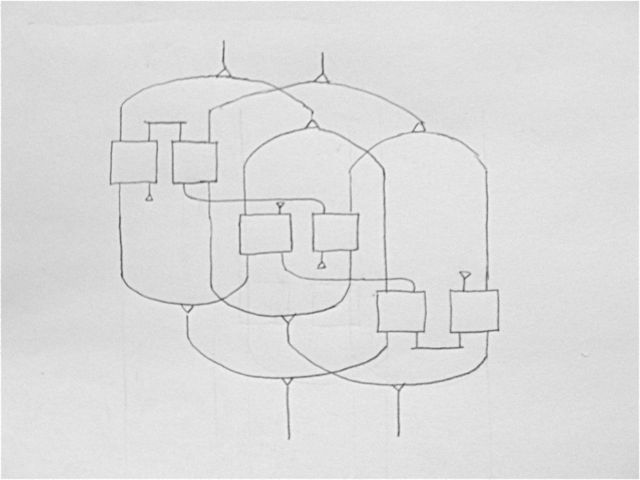
\includegraphics[scale=0.5]{./threeboxes.png}
\end{center}

\end{proof}



% \iflmcs\else\let\oldurl\url\renewcommand{\url}[1]{\hfill\break\oldurl{#1}}\fi
%
% \bibliographystyle{alpha}
% \bibliography{di-biblio}

\end{document}